\documentclass[aspectratio=169]{beamer}

\usepackage{cmap}
\usepackage{tikz}
\usepackage{array}
\usepackage{multicol}
\usepackage{booktabs}
\usepackage{csquotes}
\usepackage{amssymb,amsfonts,amsmath,bbm}

\usecolortheme{beaver}
\usefonttheme[onlymath]{serif}
\setbeamertemplate{navigation symbols}{}
\setbeamertemplate{footline}[page number]
\setbeamertemplate{blocks}[rounded=true,shadow=true]
\setbeamersize{text margin left=0.5cm,text margin right=0.5cm}
\setbeamerfont{author}{size=\normalsize}
\setbeamerfont{institute}{size=\normalsize}
\setbeamerfont{date}{size=\normalsize}

\title{Image Plagiarism Detection with Equivariant Encoders}
\author{
    Denis Gudkov\\
    Consultant: Daniil Dorin\\
    Advisor: Andrey Hrabovoy
}
\institute{
    Course: My first scientific paper\\
    Intelligent Systems Department, MIPT
}
\date{2026}

\begin{document}

% ---------------------------------------------------------------
\begin{frame}
    \thispagestyle{empty}
    \maketitle
\end{frame}

% ---------------------------------------------------------------
\begin{frame}{Goals}
    Plagiarists modify images by rotating, reflecting, shifting, and re-compressing them.
    A good detector must stay invariant to these transformations.
    \begin{block}{Hypothesis}
        Embedding exact $G$-invariance ($G \in \{D_4, SE(2)\}$) into a ViT encoder reduces FPR and raises Recall on geometric transformations from $G$, compared to a non-equivariant ViT-Tiny/16 trained with geometric augmentation.
    \end{block}
    \begin{block}{Problem}
        Standard ViTs have no geometric invariance; augmentation only covers group orbits stochastically and gives no guarantee on unseen transforms.
    \end{block}
    \begin{block}{Solution}
        \begin{enumerate}[1)]
            \item Build a siamese detector with encoders spanning $D_4$, $SE(2)$.
            \item Train each with and without geometric augmentations.
            \item Evaluate FPR and Recall on balanced DomainNet.
        \end{enumerate}
    \end{block}
\end{frame}

% ---------------------------------------------------------------
\begin{frame}[shrink=5]{Central Idea - Equivariant Encoders}
    Let $G$ act on the image space $\mathcal{X}$ and let $\rho \colon G \to \mathrm{GL}(d)$ be a linear representation of $G$ on $\mathbb{R}^d$. An encoder $\phi \colon \mathcal{X} \to \mathbb{R}^d$ is \emph{$G$-equivariant} if
    \[
      \phi(g \cdot x) = \rho(g)\, \phi(x) \quad \forall x \in \mathcal{X},\ \forall g \in G.
    \]
    % \emph{$G$-invariance} is the \emph{special case} of the trivial representation $\rho(g) = I_d$, i.e.\ $\phi(g \cdot x) = \phi(x)$; then $\phi$ is constant on each orbit $G\!\cdot\!x = \{ g \cdot x : g \in G \}$.
    \vspace{-0.6\baselineskip}
    \begin{columns}[t]
    \begin{column}[t]{0.5\textwidth}
        \vspace{0pt}% anchor column content to the top
        \begin{enumerate}[1)]
            \item Inputs: pair $(x_1, x_2)$; label $y \in \{0,1\}$.
            \item Encoder: $\phi_{\theta}$, shared, $G$-invariant.
            \item Head: symmetric fusion $h_{\psi}$, MLP.
            \item Loss: weighted BCE $+\,\lambda\,\mathcal{L}_{\mathrm{contr}}^{L^2}$.
            \item Groups: $D_4$ (Octic), $SE(2)$ (Harmformer).
        \end{enumerate}
    \end{column}
        \begin{column}[t]{0.5\textwidth}
            \vspace{0pt}
            \begin{figure}
                \centering
                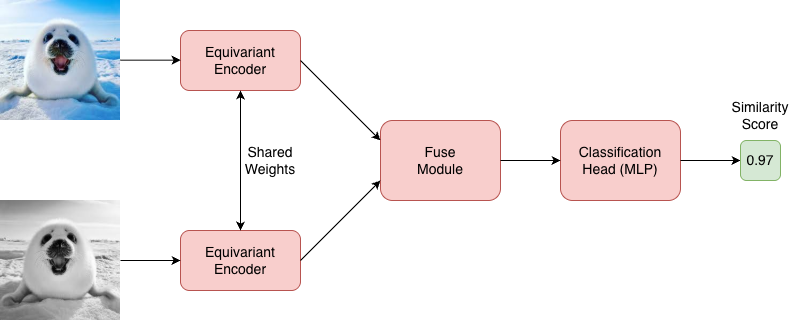
\includegraphics[width=\linewidth,height=0.34\textheight,keepaspectratio]{siamese-equivariant-pipeline}
                \caption{Siamese pipeline: shared equivariant encoder, fuse module, classification head $\to$ similarity score.}
            \end{figure}
        \end{column}
    \end{columns}
\end{frame}

% ---------------------------------------------------------------
\begin{frame}{Related Work}
    \begin{enumerate}[1)]
        \item \textbf{Bromley et al., 1993} --- siamese networks with shared weights and learned pairwise distance.
        \item \textbf{Dosovitskiy et al., 2021} --- Vision Transformer (ViT): image patches as tokens, transformer encoder, state-of-the-art on ImageNet at scale; foundation for ViT backbones in vision.
        \item \textbf{Nordstr\"{o}m et al., 2025 (Octic ViT)} --- $D_4$-equivariant ViT; 40\% FLOPs reduction.
        \item \textbf{Karella et al., 2024 (Harmformer)} --- $SE(2)$-equivariance via circular harmonic filters.
    \end{enumerate}
\end{frame}

% ---------------------------------------------------------------
\begin{frame}{Problem Statement}
    \textbf{Research hypothesis.} For each $G \in \{D_4, SE(2)\}$, let $\phi^{G}$ be a $G$-invariant ViT encoder trained with non-group augmentations only, and $\phi^{\mathrm{aug}}$ a ViT-Tiny/16 trained with non-group + group-$G$ augmentations. Then
    \[
        \mathrm{FPR}(\phi^{G}) \leq \mathrm{FPR}(\phi^{\mathrm{aug}}),\quad
        \mathrm{Recall}(\phi^{G}) \geq \mathrm{Recall}(\phi^{\mathrm{aug}}).
    \]
\end{frame}
% ---------------------------------------------------------------
\begin{frame}{Solution}
    \textbf{Model.} Siamese detector with shared $G$-invariant $\phi_{\theta}$ and symmetric head $h_{\psi}$. 
    
    Let $z_i = \phi_{\theta}(x_i)$; build pair features
    \[
        \delta = |z_1 - z_2|,\qquad
        p = z_1 \odot z_2\ \text{(element-wise)},\qquad
        v = \bigl[ u_{\delta}(\delta)\,;\, u_p(p) \bigr] \in \mathbb{R}^{2d},
    \]
    The \emph{fusion} MLP is $w_{\psi} \colon \mathbb{R}^{2d} \to [0,1]$, $w_{\psi}(v) = \sigma\Bigl( c^\top \mathrm{ReLU}\bigl( A v + b \bigr) + d \Bigr)$

    The detector output is 
    \[
        f_{\theta}(x_1, x_2) = w_{\psi}(v) = h_{\psi}\bigl(\phi_{\theta}(x_1), \phi_{\theta}(x_2)\bigr), \qquad \phi_{\theta}(g \cdot x) = \phi_{\theta}(x)\ \forall g \in G.
    \]
    \textbf{Loss.} $\mathcal{L} = \mathcal{L}_{\mathrm{BCE}} + \lambda\,\mathcal{L}_{\mathrm{contr}}^{L^2}$, where $z_i = \phi_{\theta}(x_i)$ and
    \[
        \mathcal{L}_{\mathrm{contr}}^{L^2}(z_1, z_2, y) = y\,\|z_1{-}z_2\|_2^2 + (1{-}y)\,\max(0, m - \|z_1{-}z_2\|_2)^2.
    \]

\end{frame}

% ---------------------------------------------------------------
% Slide 1: Computational Experiment
% ---------------------------------------------------------------
\begin{frame}{Computational Experiment}
    \textbf{Encoders.}
    ViT-Tiny/16 (baseline), OcticViT ($D_4$), Harmformer ($SE(2)$).
    \medskip

    \textbf{Setup.}
    \begin{itemize}
        \item Training set: COCO\,2017 (\textasciitilde118K images).
        \item Test set: DomainNet, 6 domains, 1\,200 pairs (100 pos + 100 neg per domain).
        \item Augmentation pipeline (each transform sampled independently, $p=0.3$):\\
              \textit{Non-group} (shared, all runs): {\small CJ, GBlur, GN, JPEG, WM.}\\
              \textit{Group} (added to ViT-Tiny/16 per comparison):\\
              {\small $D_4$: R90/180/270, HFlip, VFlip.}\\
              {\small $SE(2)$: R90/180/270, HFlip, VFlip, Crop, Scale.}
    \end{itemize}
\end{frame}

% Slide 2: Error Analysis \& Ablation
\begin{frame}{Error Analysis}
    \begin{columns}[t,onlytextwidth]
    \begin{column}[t]{0.50\textwidth}
        \textbf{Per-group comparison.}
        For each $G \in \{D_4, SE(2)\}$:
        \begin{enumerate}[1)]
            \item Train $\phi^{G}$ with non-group augs only.
            \item Train ViT-Tiny/16 with non-group + block-$G$ augs.
            \item Full ROC and PR curves; report AUC.
        \end{enumerate}
        Non-group augs (shared): CJ, GBlur, GN, JPEG, WM.

        \medskip
        \textbf{Per-class evaluation.}\\
        At test time, generate positive pairs using a single known
        augmentation. Report FPR and Recall separately for each
        transform class (heatmap: encoder $\times$ augmentation).    \end{column}
    \begin{column}[t]{0.50\textwidth}
        \begin{figure}[h]
            \centering
            \includegraphics[width=0.92\textwidth]{example-image-a}
            \caption{\small ROC curves per encoder (placeholder).}
        \end{figure}
        \vspace{-0.3cm}
        \begin{figure}[h]
            \centering
            \includegraphics[width=0.92\textwidth]{example-image-b}
            \caption{\small Per-class Recall heatmap (placeholder).}
        \end{figure}
    \end{column}
    \end{columns}
\end{frame}

\begin{frame}{Models, dataset, criteria}
    \begin{table}
    \centering
    \small
    \begin{tabular}{@{}llcc@{}}
    \toprule
    Encoder & Group augs given to ViT-Tiny/16 & FPR & Recall \\
    \midrule
    \multicolumn{4}{@{}l}{\textit{Comparison 1: $G = D_4$}} \\
    \quad ViT-Tiny/16 + $D_4$ augs       & R90/180/270, HFlip, VFlip & --- & --- \\
    \quad OcticViT (no group augs)        & ---                       & --- & --- \\
    \midrule
    \multicolumn{4}{@{}l}{\textit{Comparison 2: $G = SE(2)$}} \\
    \quad ViT-Tiny/16 + $SE(2)$ augs     & R90/180/270, HFlip, VFlip, Crop, Scale & --- & --- \\
    \quad Harmformer (no group augs)      & ---                       & --- & --- \\
    \bottomrule
    \end{tabular}
    \end{table}
    All encoders share non-group augmentations (CJ, GBlur, GN, JPEG, WM).\\
\end{frame}

% ---------------------------------------------------------------
\begin{frame}{Results and conclusions}\label{slide:results}
    \textbf{Results.} Placeholders pending training runs:
    \begin{itemize}
        \item FPR and Recall per encoder --- \emph{to be filled}.
        \item Per-transformation Recall heatmap (encoder $\times$ aug.\ class) --- \emph{to be filled}.
        \item ROC and PR curves per comparison ($\phi^G$ vs.\ $\phi^{\mathrm{aug}}$) --- \emph{to be filled}.
    \end{itemize}
    \textbf{Expected conclusions.}
    \begin{enumerate}[1)]
        \item For each $G$, the $G$-invariant encoder trained without group augs matches or exceeds the augmented ViT-Tiny/16 in both FPR and Recall.
        \item Adding block-$G$ augs to $\phi^G$ yields no gain.

    \end{enumerate}
\end{frame}

\end{document}
